\documentclass[tikz,border=10pt]{standalone}
\usepackage{tikz}
\usetikzlibrary{arrows.meta, positioning, calc}

\begin{document}
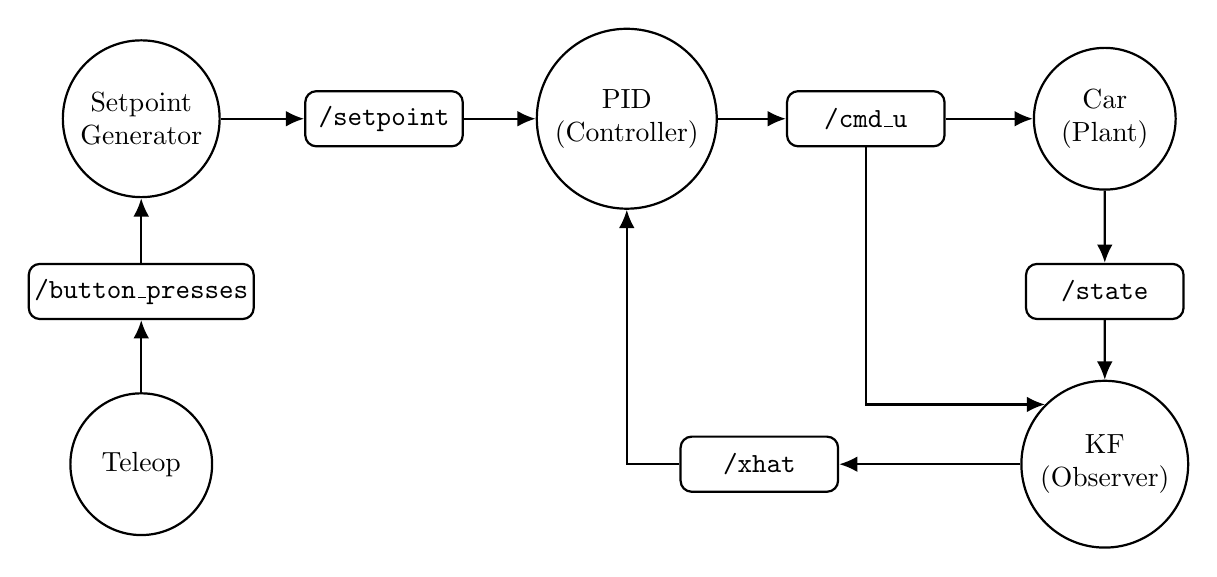
\begin{tikzpicture}[
  node/.style  = {circle, draw, thick, minimum size=18mm, align=center},
  topic/.style = {draw, thick, rounded corners, minimum height=7mm, minimum width=20mm,
                  align=center, inner sep=2pt},
  arrow/.style = {thick, -{Latex[width=2mm]}},
  node distance=3.2cm and 2.2cm
]

%--------------------------------------------------
% ROS nodes (circles)
%--------------------------------------------------
\node[node] (siggen) {Setpoint\\Generator};
\node[node, right=4.0cm of siggen] (controller) {PID\\(Controller)};
\node[node, right=4.0cm of controller] (system) {Car\\(Plant)};
\node[node, below=2.4cm of system] (observer) {KF\\(Observer)};

% Teleop node: south of Setpoint Generator, same level as observer
\node[node] (teleop) at (siggen |- observer) {Teleop};

%--------------------------------------------------
% Topics (blocks)
%--------------------------------------------------
\node[topic] (t_setpoint) at ($(siggen)!0.5!(controller)$)
  {\texttt{/setpoint}};

\node[topic] (t_cmd) at ($(controller)!0.5!(system)$)
  {\texttt{/cmd\_u}};

\node[topic] (t_state) at ($(system)!0.5!(observer)$)
  {\texttt{/state}};

% feedback topic
\node[topic, left=2.3cm of observer.west] (t_xhat)
  {\texttt{/xhat}};

% button presses topic between Teleop and Setpoint Generator
\node[topic] (t_buttons) at ($(teleop)!0.5!(siggen)$)
  {\texttt{/button\_presses}};

%--------------------------------------------------
% Connections
%--------------------------------------------------

% button_presses: teleop -> (topic) -> siggen (to south of siggen)
\draw[arrow] (teleop.north) -- (t_buttons.south);
\draw[arrow] (t_buttons.north) -- (siggen.south);

% setpoint
\draw[arrow] (siggen.east) -- (t_setpoint.west);
\draw[arrow] (t_setpoint.east) -- (controller.west);

% cmd_u
\draw[arrow] (controller.east) -- (t_cmd.west);
\draw[arrow] (t_cmd.east) -- (system.west);

% cmd_u branch to KF (south of /cmd_u -> northwest of KF)
\draw[arrow]
  (t_cmd.south)
  |- (observer.north west);

% state
\draw[arrow] (system.south) -- (t_state.north);
\draw[arrow] (t_state.south) -- (observer.north);

% xhat feedback
\draw[arrow] (observer.west) -- (t_xhat.east);
\draw[arrow] (t_xhat.west) -| (controller.south);

\end{tikzpicture}
\end{document}
